
\section{Question 2}
\label{part2}
\begin{itemize} 
\item Collection 1: Extract all the unique terms and their frequency from the 10000 files

\item Collection 2: Extract all the unique terms and their frequency of the 10000 files after 
	  running boilerpipe.
\item Construct a table with the top 50 terms from each collection.
	  - Find a common stop word list. How many of the 50 terms are on that stop word list?
\item For both collections, construct a graph with the x-axis as word rank,and y-axis as word frequency.
	  - Do either follow a Zipf distribution? Support your answer.
\end{itemize}

\subsection{Solution}

Each line of text file are parsed by splitting words on space and constructed dictionary to get the unique word list.
Here is the Python program which calculates top 50 unique word frequencies.

\lstinputlisting[language=Python,breaklines = true,frame=single,caption={Python program for calculating unique words frequency}, label=lst:q1-1,captionpos=b,numbers=left,showspaces=false,showstringspaces=false,basicstyle=\footnotesize]{getuniquefromText.py}
\newpage
\begin{table}
\caption{Rank, term and frequency from jusText file}
\begin{center}
  \begin{tabular}{ c | c | c }
    \hline
    RANK & TERM & FREQUENCY \\ \hline
1 & the  &  1164 \\ \hline
2 & and & 925 \\ \hline
3 & to & 809 \\ \hline
4 & of & 899 \\ \hline
5 & a  & 771 \\ \hline
6 & you & 625 \\ \hline
7 & I & 500 \\ \hline
8 & is & 423 \\ \hline
9 & that  & 304 \\ \hline
10 & you  & 289 \\ \hline
11 & for & 280 \\ \hline
12 & it &  253 \\ \hline
13 & with  &  249 \\ \hline
14 & or & 245 \\ \hline
15 & on & 229 \\ \hline
16 & this & 222 \\ \hline
17 & we & 221 \\ \hline
18 & s  & 218 \\ \hline
19 & your  & 201 \\ \hline
20 & as & 176 \\ \hline
21 & from &   170 \\ \hline
22 & domain & 150 \\ \hline
23 & will   & 146 \\ \hline
24 & are & 140 \\ \hline
25 & not & 137 \\ \hline
26 & by & 131 \\ \hline
27 & be & 120 \\ \hline
28 & at & 117 \\ \hline
29 & have &  114 \\ \hline
30 & all  & 110 \\ \hline
31 & can & 108 \\ \hline
32 & my & 108 \\ \hline
33 & t &  99 \\ \hline
34 & my & 98 \\ \hline
35 & about & 94 \\ \hline
36 & when &  92 \\ \hline
37 & like & 86 \\ \hline
38 & use & 85 \\ \hline
39 & so & 84 \\ \hline
40 & more & 83 \\ \hline
41 & but & 80\\ \hline
42 & do & 79 \\ \hline
43 & any & 79 \\ \hline
44 & about & 77 \\ \hline
45 & her & 77 \\ \hline
46 & just & 76 \\ \hline
47 & one& 70 \\ \hline
48 & who & 68 \\ \hline
49 & has & 67 \\ \hline
50 & if &  67 \\
    \hline
  \end{tabular}
  \label{table:textFiles}
\end{center}
\end{table} 

\begin{table}
\caption{ Top 50 terms extracted from HTML files}
\begin{center}
\begin{tabular}{ c | c | c }
 \hline
 RANK & TERM & FREQUENCY \\ \hline
1 &div &5921\\ \hline
2 &= &3933\\ \hline
3 &the &3711\\ \hline
4 &<a &3511\\ \hline
5 &to &3408\\ \hline
6 &and &3390\\ \hline
7 &a &3270\\ \hline
8 &of &3110\\ \hline
9 & \{&3032\\ \hline
10 &\textless li \textgreater \textless a &2913\\ \hline
11 &\textless span &2878\\ \hline
12 &\textless /div \textgreater &2773\\ \hline
13 &in &2683\\ \hline
14 &\{. &2583\\ \hline
15 &for &2480\\ \hline
16 &- &2310\\ \hline
17 & \textless li &2237\\ \hline
18 &at &2137\\ \hline
19 &var &2031\\ \hline
20 &point:false, &1997\\ \hline
21 &on &1896\\ \hline
22 &+ &1793\\ \hline
23 &\textless /div \textgreater &1633\\ \hline
24 &is &1489\\ \hline
25 & target='self' & 1211\\ \hline
26 &? &1031\\ \hline
27 &position:'left'\}, &937\\ \hline
28 &yous &820\\ \hline
29 &your &708\\ \hline
30 & \textless /li \textgreater&681\\ \hline
31 &class="user-in" &608\\ \hline
32 &with &585\\ \hline
33 &I &565\\ \hline
34 &user &550\\ \hline
35 &target='' &520\\ \hline
36 &\&amp; &482\\ \hline
37 &2014 &472\\ \hline
38 & \textless /a \textgreater &460\\ \hline
39 &December &452\\ \hline
40 &0 &400\\ \hline
41 &rel='fll' &368\\ \hline
42 &\textless img &355\\ \hline
43 &onclick="return &352\\ \hline
44 &if &350\\ \hline
45 & follow:false,&348\\ \hline
46 &class="hight" &337\\ \hline
47 &type="hidden" &333\\ \hline
48 &The &322\\ \hline
49 &alt &306\\ \hline
50&class="high &296\\ \hline
    \hline
  \end{tabular}
\end{center}
\label{table:htmlFiles}
\end{table}

\subsection{Find terms which are common in stop words list:}

\begin{itemize}
\item 16 terms from Table \ref{table:textFiles} are common with the stop words list that I retrieved from \url{http://www.ranks.nl/stopwords}.
\item 38 terms from Table \ref{table:htmlFiles} are common with the stop words list. 
\item Stop words are listed in the file stop-words.txt.
\item Both collections before and after running boilerpipe are plotted on a single graph.
Below is the R code which is used to plot the data.
\end{itemize}

\lstinputlisting[language=Python,breaklines = true,frame=single,caption={R program to plot both collections}, label=lst:q1-1,captionpos=b,numbers=left,showspaces=false,showstringspaces=false,basicstyle=\footnotesize]{Plot.R}


\begin{itemize}
\item As shown in the figure below, both plots follow Zipfian Distribution\cite{Zipf}.
\item The frequency of each word is close to inversely proportional to its rank in the frequency table. This is known as the power law.
\item As shown in the figure below, most frequent word occurs approximately twice as the second most frequency word.
\end{itemize}	        
\begin{figure}[ht]
	\begin{center}
		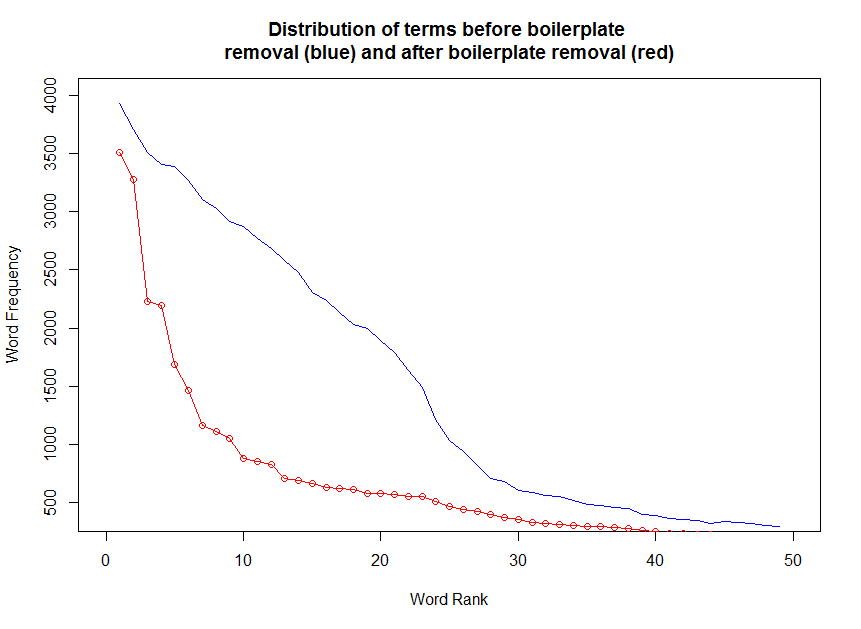
\includegraphics[scale=0.40]{Rplotfinal.png}
		\caption{Graph with x-axis as word rank , and y-axis as word frequency}
		\end{center}
\end{figure}